%%
%
% ARQUIVO: main.tex
%
% VERSÃO: 1.0
% DATA: Maio de 2016
% AUTOR: Coordenação de Trabalhos Especiais SE/8
% 
%  Arquivo tex principal do documento de Projeto de Fim de Curso (PFC).
%  Este arquivo SÓ PRECISA SER MODIFICADO NA PARTE DE CONTEÚDO:
%
%    a. colocar um \include{•} para cada capítulo do documento de PFC.
%
%%

% -----
% CLASSE DO DOCUMENTO DE PFC
% -----
\documentclass{pfc}
\usepackage{pgfgantt}

% -----
% PACOTES LATEX USADOS NO DOCUMENTO DE PFC
% -----
\usepackage[brazilian]{babel}
\usepackage[utf8]{inputenc}
\usepackage[T1]{fontenc}

\usepackage{amsmath}
\usepackage{graphicx}
\usepackage{tabularx}
\usepackage{float}
\usepackage{color}
\usepackage{amsfonts,amssymb}
\usepackage[authoryear]{natbib}

\usepackage{enumitem}
\usepackage{rotating}
\usepackage{lipsum}
\usepackage{lastpage}
\usepackage{stringstrings}
\usepackage{pgffor}
\usepackage{pdftexcmds}

% -----
% MARGENS DO DOCUMENTO DE PFC
% -----
\usepackage{geometry}
\geometry{
	a4paper,
	total={210mm,297mm},
	left=25mm,
	right=25mm,
	top=25mm,
	bottom=30mm,
	textwidth=160mm,
	textheight=242mm,
	headheight=0mm,
	headsep=0mm,
}

% -----
% DECLARAÇÕES AUXILIARES PARA REFERÊNCIAS
%
%  Diferencia \citet e \citep de acordo com a NBR 10520:2002
% -----
\DeclareRobustCommand{\NATand}{;}
\DeclareRobustCommand{\NATetal}{et~al.}
\makeatletter
\renewcommand{\NAT@nmfmt}[1]{%
  \ifNAT@swa\expandafter\MakeUppercase
  \else\DeclareRobustCommand{\NATand}{ e}\expandafter\@firstofone\fi{{\NAT@up #1}}%
}
\makeatother

% -----
% AMBIENTE DE FIGURAS DE PFC
%
%  A classe do documento está configurada SOMENTE para figuras no formato EPS.
%  Logo, use PREFERENCIALMENTE este tipo de arquivo.
%
%    a. os arquivos das figuras devem estar no diretório 'img'
% -----
\graphicspath{{./img/}}

% -----
% INÍCIO DO DOCUMENTO DE PFC
% -----
\begin{document}

% -----
% PARTE PRÉ-TEXTUAL DE PFC
%
% Alterar o CONTEÚDO dos arquivos siglas.tex E pre-texto.tex
% -----
%%
%
% ARQUIVO: dados-pfc.tex
%
% VERSÃO: 1.0
% DATA: Maio de 2016
% AUTOR: Coordenação de Trabalhos Especiais SE/8
% 
%  Arquivo tex com os dados acerca do documento de PFC e da apresentação.
%
%   nos campos que definem nomes (autor; orientador; co-orientador; membros da banca)
%   É PRECISO usar os COMANDOS LaTeX para acentuação, conforme abaixo:
%
%         \'a - á || \`a - à || \~a - ã || \^a - â 
%         \'e - é || \^e - ê || \'i - í 
%         \'o - ó || \~o - õ || \^o - ô 
%         \'u - ú || \"u - ü
%
%%

%%% AUTORES DO PFC (Nome completo)
% ---
%  aceita até 03 autores (de autorI até autorIII)
%    a. preencher sucessivamente a partir de autorI
%    b. REMOVER as definições não necessárias
% ---
\autorI{Pedro Igor de Ara\'ujo Oliveira}
\autorII{Bruno Vieira Costa}
\autorIII{Lucas Ricarte Rogério Teixeira}

%%% POSTOS DOS AUTORES DO PFC
% ---
%  aceita os postos de até 03 autores (de postoautorI até postoautorIII)
%    a. preencher sucessivamente a partir de postoautorI (que deve ser o posto de autorI)
%    b. se o autorX É CIVIL, NÃO DEFINIR postoautorX (remover a linha de definição)
%    c. se o autorX É MILITAR, DEFINIR postoautorX com UMA das seguintes ALTERNATIVAS: Alu / 1 Ten / Cap
% ---
\postoautorI{1 Ten}

%%% TITULO DO PFC
\titulo{Ferramentas de classificação multidimensional para plataforma de auxílio ao aprendizado}

%%% DATA DA APRESENTAÇÃO (formato {dd}{Mmmmm}{aaaa})
\datadefesa{14}{Maio}{2018}

%%% ORIENTADOR DO PFC
% ---
%  CAMPO 1: P (para Prof.); PA (para Profa.); ou qualquer coisa (inclusive VAZIO) - o que for escrito aparecerá no documento
%  CAMPO 2: Nome completo
%  CAMPO 3: D (para D.Sc.); P (para Ph.D.); M (para M.Sc.) ou qualquer coisa (inclusive VAZIO) - o que for escrito aparecerá no documento
%  CAMPO 4: Instituição (com "do / da")
% ---
\orientador{P}{Alex de Vasconcellos Garcia}{D}{do IME}

%%% CO-ORIENTADOR DO PFC
% ---
%  se não houver co-orientador, REMOVA ESTA LINHA
%  preenchimento idêntico a \orientador{}{}{}{}
% ---
% \coorientador{P}{Nome Completo do Co-orientador}{P}{do IME}

%%% NÚMERO DA ENTRADA DA BIBLIOTECA (pegar na Biblioteca do IME)
\biblioref{004.69}{S586e}

%%% PALAVRAS-CHAVES DO PFC
% ---
%  devem ser separadas por vírgula e É OBRIGATÓRIO ter pelo menos uma
% ---
\palavraschaves{Classificação de texto, Processamento de linguagem natural, Ferramenta de auxílio ao aprendizado, Aprendizado de máquina}

%%% OUTROS MEMBROS DA BANCA DO PFC
% ---
%  aceita até mais 05 membros (de membrobancaI até membrobancaV)
%    a. preencher sucessivamente a partir de membrobancaI
%    b. REMOVER as definições não necessárias
%
%  cada membro tem preenchimento idêntico a \orientador{}{}{}{}
% ---
\membrobancaI{P}{Ronaldo Ribeiro Goldschmidt}{D}{da PUC-RJ}
\membrobancaII{P}{Julio Cesar Duarte}{D}{da PUC-RJ}
%\membrobancaIII{}{Nome do Membro da Banca 3}{}{da COPPE/UFRJ}
%\membrobancaIV{}{Nome do Membro da Banca 4}{}{da UNIRIO}
%\membrobancaV{}{Nome do Membro da Banca 5}{}{da UERJ}

%%
%
% ARQUIVO: pre-texto.tex
%
% VERSÃO: 1.0
% DATA: Maio de 2016
% AUTOR: Coordenação de Trabalhos Especiais SE/8
% 
%  Arquivo tex para a criação da parte pré-textual do documento de Projeto de Fim de Curso.
%
%%


% -----
% PÁGINA DE CAPA DO DOCUMENTO DE PFC
% -----
\makecapa

% -----
% PÁGINA DE TÍTULO DO PFC
% -----
\prepareadvisors
\maketitle

% -----
% PÁGINA DE CRÉDITOS DO DOCUMENTO DE PFC
% -----
\makecredits

% -----
% PÁGINA DE FOLHA DE ASSINATURAS
% -----
\preparemembers
\approvalpage

% -----
% PÁGINA DE DEDICATÓRIA (OPCIONAL, ie. pode remover toda a página)
% -----
%%% DEDICATÓRIA - PREENCHER...
% \dedicatoria{%
% Ao Instituto Militar de Engenharia, alicerce da minha formação e aperfeiçoamento.
% }%
% \makededication

% -----
% PÁGINA DE AGRADECIMENTOS (OPCIONAL, ie. pode remover toda a página)
% -----
%%% AGRADECIMENTOS - PREENCHER...
\agradecimentos{%
Agradecemos a todas as pessoas que nos incentivaram, apoiaram e possibilitaram esta oportunidade de ampliar nossos horizontes. \\
\indent
Em especial ao Professor Orientador Dr. Alex Garcia.
}%
\makethanks

% -----
% PÁGINA DE EPÍGRAFE (OPCIONAL, ie. pode remover toda a página)
% -----
%%% EPÍGRAFE - PREENCHER...
\epigrafe{%
Not everything that can be counted counts; and not everything that counts can be counted.}%
\autorepigrafe{%    %% Se não tem autor, coloque "Anônimo"
Anônimo
}%
\makeepigraph

% -----
% PÁGINA DE SUMÁRIO
% -----
\tableofcontents

% -----
% PÁGINAS DE LISTAS DE FIGURAS E DE TABELAS
% se a Dissertação não possui figuras e/ou tabelas, REMOVA O COMANDO CORRESPONDENTE
% -----
\listoffigures
\listoftables

% -----
% PÁGINA DE LISTA DE SIGLAS
% se a Dissertação não possui siglas, REMOVA TODA A PÁGINA
% -----
%%% SIGLAS - PREENCHER...
\acronimo{API}{\textit{Application programming interface}}
\acronimo{AWS}{\textit{Amazon Web Services}}
\acronimo{CNN}{\textit{Convolutional Neural Network}}
\acronimo{CPU}{\textit{Central processing unit}}
\acronimo{EAD}{Ensino à distância}
\acronimo{GPU}{\textit{Graphics Processing Unit }}
\acronimo{HTML}{\textit{Hypertext Markup Language}}
\acronimo{HTTP}{\textit{Hypertext Transfer Protocol}}
\acronimo{IA}{Inteligência Artificial}
\acronimo{JSON}{\textit{JavaScript Object Notation}}
\acronimo{LSTM}{\textit{Long Short Term Memory}}
\acronimo{NB}{\textit{Naive Bayes}}
\acronimo{NN}{\textit{Neural Network}}
\acronimo{RNN}{\textit{Recurrent Neural Network}}
\acronimo{SepCNN}{\textit{Separable Depthwise Convolutional Neural Network}}
\acronimo{SVM}{\textit{Support Vector Machine}}
\acronimo{TF-IDF}{\textit{Term Frequency-Inverse Document Frequency}}
\acronimo{VM}{\textit{Virtual Machine}}
\listofnicks

% -----
% PÁGINA DE LISTA DE ABREVIATURAS
% se a Dissertação não possui abreviaturas ou símbolos, REMOVA TODA A PÁGINA
% -----
%%% ABREVIATURAS - PREENCHER...
%\abreviatura{Ja}{jacobiano}
%\abreviatura{JS}{fluxo secundário (difusivo)}
%\abreviatura{M}{número de Mach}
%
%%%% SÍMBOLOS - PREENCHER...
%\simbolo{$\Phi$}{termo de dissipação viscosa}
%\simbolo{$\Gamma$}{coeficiente de difusão efetivo}
%\simbolo{$\alpha$}{fator de sub-relaxação}
%\simbolo{$\phi$}{variável dependente da equação diferencial geral}

%\listofsymbols

% -----
% PÁGINA DE RESUMO
% -----
%%% RESUMO - PREENCHER...
\resumo{%
Ferramentas de auxílio ao aprendizado são usadas nas mais diversas etapas da educação formal ou informal. Estas ferramentas costumam empregar diversas tecnologias. Dentre elas, pode-se incluir a classificação de documentos, pois essas plataformas são, em geral, grandes agregadoras de conteúdo de ensino. Para uma melhor acessibilidade de todo esse conteúdo, é necessário que ele seja categorizado, o que nem sempre é viável de ser realizado manualmente devido ao grande volume e a necessidade de conhecimento técnico sobre os assuntos abordados. Nesse contexto, pode ser aplicada a Classificação Automática de Documentos.\\
\indent
Este trabalho tem como objetivo analisar e implementar modelos consagrados de classificação de texto, aplicando-os para a classificação de enunciados de questões em avaliações de ensino segundo seus assuntos. A partir da exploração dessas técnicas, desenvolveu-se um modelo híbrido de classificador especializado em enunciados de questões.}%
\makeresumo

% -----
% PÁGINA DE ABSTRACT
% -----
%%% ABSTRACT - PREENCHER...
\abstract{%
Learning aid tools are used in the most diverse stages of formal or informal education. These tools usually employ various technologies. Among them, one can include the classification of documents, since these platforms are, in general, great aggregators of teaching content. For a better accessibility of all this content, it needs to be categorized, which is not always feasible to be done manually due to the large volume and the need for technical knowledge on the issues addressed. In this context, it's interesting to apply the Automatic Document Classification.\\
\indent
This work aims to analyze and implement established text classification models, applying them to the classification of question statements in teaching assessments according to their subjects. From the exploration of these techniques, a hybrid classifier model was developed that specializes in question statements.
}%
\makeabstract

\parindent 0.75cm

% -----
% PARTE DE CONTEÚDO DE PFC
%
%  Escrever cada capitulo do documento de PFC em um arquivo .tex separado.
%  Adicionar os arquivos .tex ao documento com comando \include{•}
% -----
%%
%
% ARQUIVO: cap-01.tex
%
% VERSÃO: 1.0
% DATA: Maio de 2016
% AUTOR: Coordenação de Trabalhos Especiais SE/8
% 
%  Arquivo tex de exemplo de capítulo do documento de Projeto de Fim de Curso.
%
% ---
% DETALHES
%  a. todo capítulo deve começar com \chapter{•}
%  b. usar comando \noindent logo após \chapter{•}
%  c. citações para referências podem ser
%       i. \citet{•} para citações diretas (p. ex. 'Segundo Autor (2015)...'
%       ii. \citep{•} para citações indiretas (p. ex. '... (AUTOR, 2015)...'
%  d. notas de rodapé devem usar dois comandos
%       i. \footnotemark para indicar a marca da nota no texto
%       ii. \footnotetext{•}, na sequência, para indicar o texto da nota de rodapé
%  e. figuras devem seguir o exemplo
%       i. devem ficar no diretório /img e devem ser no formato EPS
%  f. tabelas devem seguir o exemplo
%  g. figuras e tabelas podem ser colocadas em orientação landscape
%       i. figuras: usar \begin{sidewaysfigure} ... \end{sidewaysfigure}
%                   em vez de \begin{figure} ... \end{figure}
%       ii. tabelas: usar \begin{sidewaystable} ... \end{sidewaystable}
%                    em vez de \begin{table} ... \end{table}
%  h. toda figura e tabela deve ser referenciada ao longo do texto com \ref{•}
% ---
%%

\chapter{Introdução}
\noindent
O objetivo deste trabalho é desenvolver um algoritmo que classifique uma questão inédita de concurso dentre um conjunto de assuntos pré-determinados. Para atingir este objetivo, serão exploradas técnicas de aprendizado de máquina e processamento de linguagem natural.


\section{Motivação}
%porque estudar o tema é importante/relevante?

\subsection{Plataformas de auxílio ao aprendizado}
Neste relatório, será entendido por PAA qualquer software que tenha objetivo pedagógico. Existe um mercado de educação à distância (EAD) que por seu caráter remoto, propicia o uso de tecnologia digital para a facilitação do ensino.  Esse mercado tem se tornado competitivo e ganhado cada vez mais importância.

\subsection{Classificação automática de assuntos}

Será entendido por CAA qualquer método de classificação de textos exequível via software sem auxílio de um operador. Os principais métodos existentes são listados na seção de Métodos.
A CAA já é amplamente utilizada na indústria, por exemplo, em sites de notícias, gerenciadores de emails ou motores de busca.

\subsection{Loona}
Loona é um motor de busca em desenvolvimento pela empresa PaperX. Trata-se de uma ferramenta de busca de vídeos por imagem.

\begin{figure}[!ht]
	\centering
	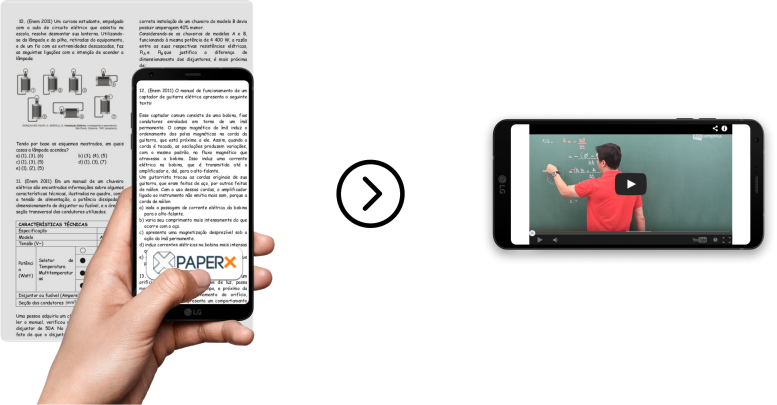
\includegraphics[width=0.4\textwidth]{figures/loona.png}   
	\caption{Funcionamento do loona}
	\label{fig:loona}
\end{figure}


\section{Objetivo}
%que tentará ser alcançado (principal e secundários)
O funcionamento do motor de busca em questão é dividido em três etapas:
\begin{itemize}
\item Reconhecimento ótico de caracteres (OCR); 
\item Classificação de texto e
\item Busca
\end{itemize}

\begin{figure}[!ht]
	\centering
	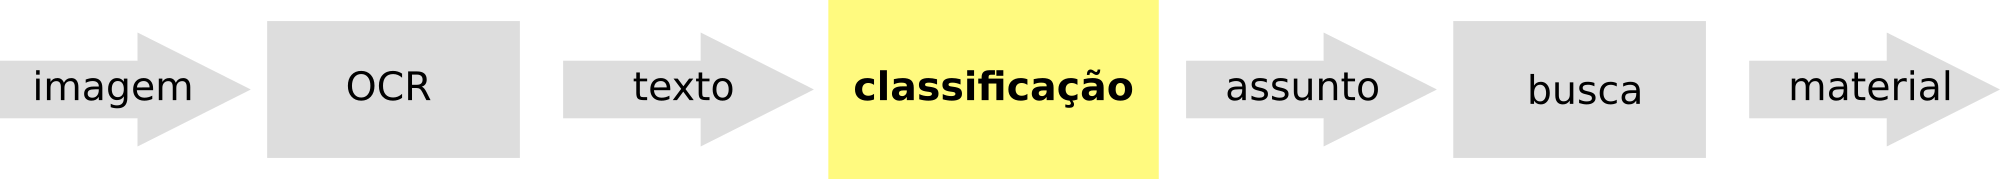
\includegraphics[width=0.4\textwidth]{figures/fluxograma.png}   
	\caption{Fluxo funcional da ferramenta}
	\label{fig:fluxograma}
\end{figure}


Este trabalho será restrito a etapa central: Classificação de texto.


% \section{Justificativa}
%a importância do trabalho no contexto institucional

\section{Metodologia}
%como o trabalho deverá ser conduzido
A primeira etapa do trabalho corresponde à obtenção de dados para serem utilizados nos algoritmos de aprendizado de máquina. Isso é feito a partir de Web scraping de questões de concursos públicos já rótuladas com os seus respectivos assuntos.

Em seguida, há uma fase de processamento de dados que remove inconsistências e prepara uma interface ideal para os algoritmos que serão aplicados posteriormente.

A terceira fase é a parte central do trabalho e consiste em explorar diferentes modelos para a classificação de questões. Cada um desses modelos possui suas particularidades com diferentes arquiteturas e hiperparâmetros para uma otimização de acordo com o contexto dos dados utilizados.

Como etapa final, a solução ótima encontrada de classificação é implementada na plataforma de auxílio ao aprendizado da paperx.com.br para o uso em ferramentas de busca.


\section{Estrutura}
%do documento
Sobre os capítulos subsequentes a seguinte distribuição de conteúdo:
\begin{itemize}
\item Capítulo 2: 
fundamentação teórica sobre cada um dos algoritmos de classificação que serão utilizados;
\item Capítulo 3:
descrição da implementação para cada uma das etapas descritas na metodologia;
\item Capítulo 4:
comparação dos resultados dos entre diferentes modelos implementados.
\end{itemize}
\chapter{Trabalhos Relacionados}
\noindent
\chapter{Obtenção das Bases}
\label{chapter:ObtencaoBases}
\noindent

A primeira etapa de implementação desenvolvida no trabalho foi a aquisição de um conjunto de questões rotuladas de acordo com seus assuntos para se viabilizar a aplicação de algoritmos de classificação. Esse conjunto de dados foi obtido por meio de \textit{web scrapping}. Posteriormente, os arquivos baixados foram filtrados e convertidos para um novo formato de maneira a se armazenar apenas os dados de interesse. Finalmente, desenvolveu-se uma interface que faz uso de todo esse conjunto de dados, tornando-o acessível para as demandas nos diferentes algoritmos de aprendizado de máquina. A figura \ref{fig:data_processing_pipeline} ilustra a sequência de operações executadas na aquisição de dados e que serão descritas em detalhes a seguir.

\begin{figure}[!ht]
	\centering
	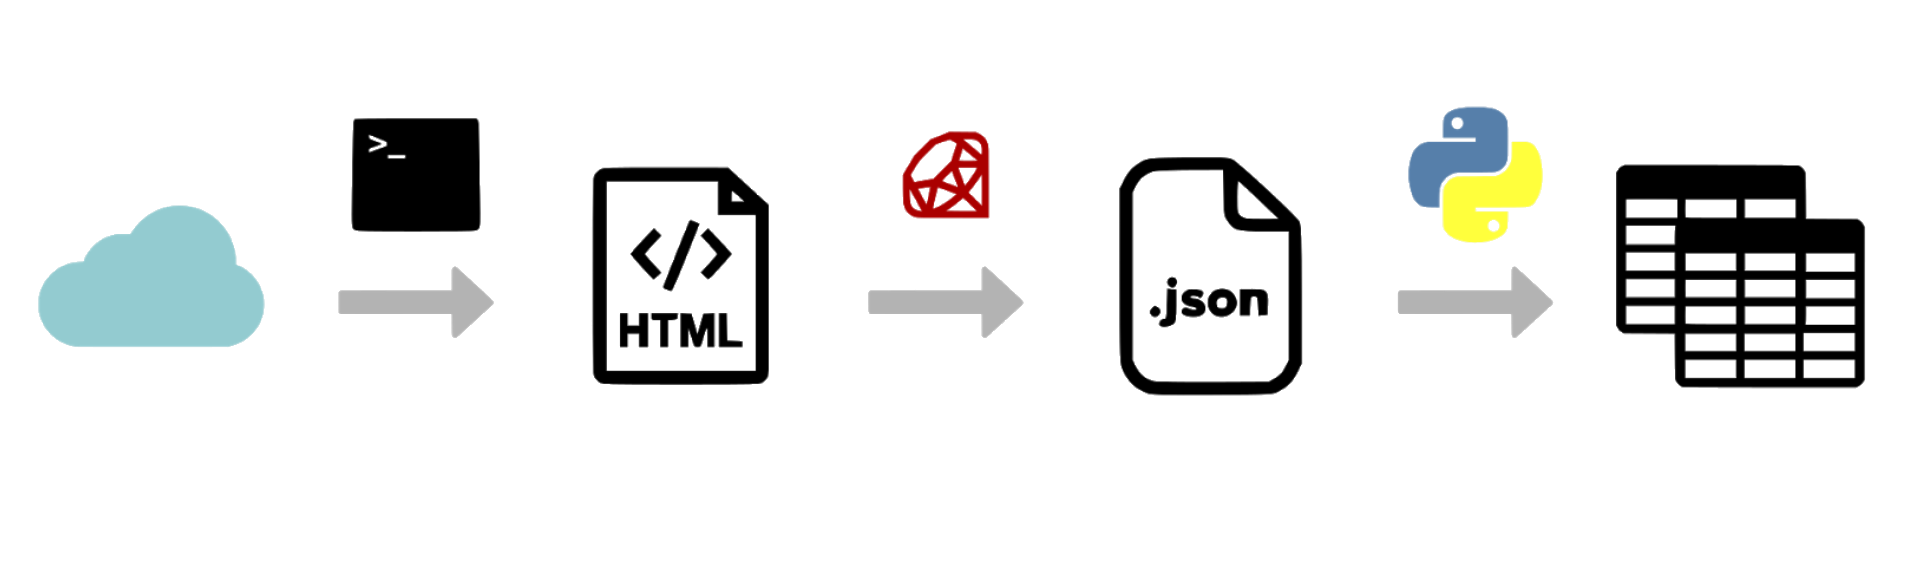
\includegraphics[width=0.9\textwidth]{figures/data_processing_pipeline.PNG}
	\caption{Sequência de operações para a aquisição de dados}
	\label{fig:data_processing_pipeline}
\end{figure}

\section{Web Scrapping}

As questões utilizadas para treinamento dos modelos classificatórios foram retiradas de um site preparatório para concursos públicos chamado “Rota dos concursos” (rotadosconcursos.com.br). Para esta tarefa, foi implementado um ruby script que simulava as requisições HTTP feitas por um navegador. Cada requisição realiza o \textit{download} de um arquivo HTML de uma página do site que contem exatamente uma questão de concurso público.

Devido à grande quantidade de questões, foi utilizado um serviço de servidores dedicados em nuvem para possibilitar as muitas horas de requisição. A quantidade de questões também impossibilitou a manipulação dos arquivos em um único diretório. Desta forma foi utilizado um esquema de subpastas enumeradas de 000 a 999 tornando a manipulação no sistema de arquivos tratável, pois os arquivos são uniformemente distribuídos nessas subpastas por meio de uma função de \textit{hash} simples. Além disso, como o gargalo são operações de entrada e saída (I/O \textit{bound}) nas requisições, foi utilizado \textit{multithreading} para otimizar o uso de CPU.
    
\section{Pré-Processamento}

Após o download em formato HTML, o conteúdo de cada página teve de ser isolado em arquivos em formato JSON. Cada arquivo continha apenas os dados referentes a uma questão, de maneira a descartar as informações referentes ao \textit{layout} da página e manter os seguintes atributos:

\begin{itemize}
\item id: Identificador único de cada questão;
\item text: Enunciado da questão;
\item subject\_path: Lista de \textit{strings} iniciada pela área de conhecimento abrangido pela questão e seguida pela hierarquia de domínios abrangidos em ordem de especificidade;
\item alternatives: Lista com o texto de cada uma das alternativas caso a questão seja de múltipla escolha;
\item image\_count: Contagem de imagens utilizadas no enunciado da questão, vale ressaltar que essa imagem pode conter até mesmo informação textual não capturada pelo atributo text;
\item concurso: Nome do concurso público do qual a questão foi extraída;
\item prova: Ano em que a prova foi aplicada;
\item banca: Banca referente ao concurso público da questão;
\item nivel: Nível de escolaridade utilizado como pré-requisito no concurso público em que questão foi obtida;
\item answer: Alternatica correspondente a resposta correta caso a questão seja de múltipla escolha.
\end{itemize}

Ao término desse pré-processamento, obteve-se um total de mais de 500 mil arquivos JSON com questões.

\section{API de dados}
\label{dataset_api}

Como uma etapa final da sequência de operações antes de se iniciar a etapa analítica, foi necessário desenvolver uma interface que fosse flexível para as diferentes demandas de dados de treinamento/validação/teste no desenvolvimento dos algoritmos de aprendizado de máquina. Para isso, foi implementada uma classe na linguagem python (mesma utilizada para na etapa seguinte) que contivesse os dados de todas as questões armazenadas inicialmente em distintos arquivos JSON em uma única estrutura de dados em memória. Para isso, utilizou-se a estrutura de um \textit{dataframe} do pacote pandas devido a sua boa performance com o uso de operações de \textit{broadcast} em um grande conjunto de dados e a sua fácil manipulação.

Além disso, foram definidos alguns parâmetros para o construtor dessa classe, de maneira a possibilitar o seu uso em diferente contextos de teste:

\begin{itemize}

  \item random\_state: Número inteiro utilizado como \textit{seed} de aleatorização quando for necessário distribuir arbitrariamente o conjunto de dados conforme é detalhado nos parâmetros \textit{frac} e \textit{subset}.
  
  \item frac: Determina a fração dos dados que vai ser carregada, possibilitando tanto um uso reduzido para maior velocidade nos testes de desenvolvimento como o uso completo para obtenção de resultados finais.
  
  \item dict\_name: Nome de um arquivo JSON utilizado como dicionário para agrupamento de assuntos. Esse parâmetro possibilita o agrupamento de assuntos similares, já que originalmente existem 133 áreas de conhecimento definidas e com grande interseção entre elas, o que inviabiliza a classificação das questões até mesmo por seres humanos especialistas, pois a classificação possuiria um caráter subjetivo. Para ilustrar a existência de domínios de conhecimento similares, pode-se citar Engenharia de Redes e Engenharia de Telecomunicações, bem como Contabilidade Privada Contabilidade Pública. Vale destacar que o fato de ser um arquivo externo usado como dicionário flexibiliza o teste de diferentes agrupamentos, permitindo a escolha de um agrupamento que resulte em uma melhor performance de classificação.
  
  \item min\_number\_per\_label: Número mínimo de amostras para cada área de conhecimento após o agrupamento, as amostras referentes a assuntos com total insuficiente são descartadas. Esse parâmetro é importante porque podem existir áreas de conhecimento com um número insuficiente de amostras para realizar o treinamento de um algoritmo de classificação.

  \item subset: Determina se o objeto a ser instanciado terá fração de dados correspondente ao treinamento, validação, teste ou todo o conjunto de dados. A divisão desses conjuntos é feita de maneira aleatória e a consistência dessa aleatorização para diferentes instâncias é determinada pelo parâmetro \textit{random\_state}.
  
\end{itemize}

Além disso, a API de dados também faz uso de cache do \textit{dataframe} base no formato de um arquivo csv para evitar a releitura das centenas de milhares de arquivos JSON sempre que for necessário criar um nova instância da classe.

Finalmente, sobre os métodos oferecidos pela API de dados, pode-se destacar a existência de métodos que retornam estruturas com dados utilizados no treinamento como o enunciado de todas as questões contendo todos o caracteres possíveis ou apenas caracteres alfabéticos, o assunto de todas questões no formato de \textit{string} ou de \textit{one-hot-encoding}. 
%Demonstra como foi realizado o trabalho
%• Pesquisas bibliográficas: sempre com as referências
%• Modelagem
%• Sistema gerado
%• Testes de desempenho/avaliação
\chapter{Fundamentação Teórica}
\label{cap:methods}
\noindent

Aprendizado de máquina é um ramo da inteligência artificial na Ciência da Computação em que se faz uso de dados para o desenvolvimento de um algoritmo por meio de etapas de treinamento. Mais especificamente no aprendizado supervisionado, estuda-se um conjunto de dados rotulados na fase de treinamento para que o algoritmo treinado possa prever um rótulo de um dado inédito baseando-se nos padrões já estudados. Para a classificação de textos em assuntos, o aprendizado supervisionado é o mais utilizado, de maneira que os rótulos correspondem aos próprios assuntos dos textos a serem utilizados no treinamento.

Contudo, uma dificuldade ao se trabalhar com um texto é o uso de uma representação computacional que seja facilmente interpretável pelos algoritmos de aprendizado de máquina. Por isso, são utilizadas representações específicas para esses algoritmos como Bag of Words e Word Embeddings que serão descritos nas seções a seguir. Posteriormente, pode-se aplicar algoritmos como, por exemplo, redes neurais que também serão descritas nas seções seguintes.

\section{Bag of Words}
%https://www3.nd.edu/~dchiang/teaching/nlp/2015/notes/chapter1v2.pdf
%https://towardsdatascience.com/machine-learning-nlp-text-classification-using-scikit-learn-python-and-nltk-c52b92a7c73a

Bag of words não se trata de um modelo de classificação por completo, mas sim de uma estratégia de representação do texto em que a sequência de palavras é desconsiderada. Dessa maneira, o texto é simplificado para uma lista de palavras distintas e a respectiva contagem de ocorrência de cada uma delas. A principal vantagem dessa estratégia é a sua simplicidade de representação computacional, sendo atrativa para a aplicação direta de algoritmos de aprendizado de máquina.

Contudo, para se obter uma melhor eficiência dessa estratégia, pode ser necessário aplicar outras técnicas que mitiguem a perda de informação causada pelo \textit{bag of words}. Uma dessas técnicas é a remoção de palavras de parada (stop words), pois essas palavras são utilizadas apenas para a conexão de ideias em uma frase como preposições, artigos e conjunções e não contribuem como fonte de informação no texto. Além disso, as palavras vazias ocorrem com alta frequência e possuem destaque ilusório na representação colapsada do bag of words. Outra técnica que também pode ser empregada é a lematização (\textit{stemming}) que corresponde a remoção dos sufixos das palavras, pois estes fazem com que palavras que deveriam ser sinônimas na representação \textit{bag of words} sejam contabilizadas separadamente. Ao remover os sufixos como gênero, tempo e número, palavras que acrescentam a mesma informação ao texto terão suas respectivas contagens somadas em uma única palavra sem os sufixos. A figura \ref{fig:nl_ex} mostra um exemplo dessas etapas de pré-processamento.

\begin{figure}[!ht]
	\centering
	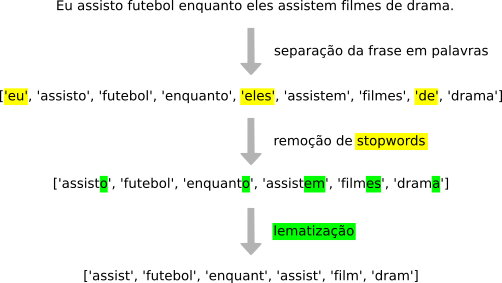
\includegraphics[width=1\textwidth]{figures/nltp_example.png}
	\caption{Etapas do processamento de linguagem natural}
	\label{fig:nl_ex}
\end{figure}

Após todas essas técnicas, pode-se extrair ainda a representação TF-IDF (\textit{term frequency-inverse document frequency}), \cite{InformationRetrievalBookChapter6}, de cada amostra de um conjunto de textos, trata-se de uma medida estatística para normalizar o peso das palavras. Nesse indicador, a relevância de uma palavra em determinado contexto é representada pelo número de vezes que a palavra nesse contexto dividido pelo número de vezes que ela aparece em todos os documentos que fazem parte do \textit{corpus} analisado. A figura \ref{fig:bow_ex} mostra um exemplo da representação de dois documentos conforme a modelagem \textit{bag of words}.

\begin{figure}[!ht]
	\centering
	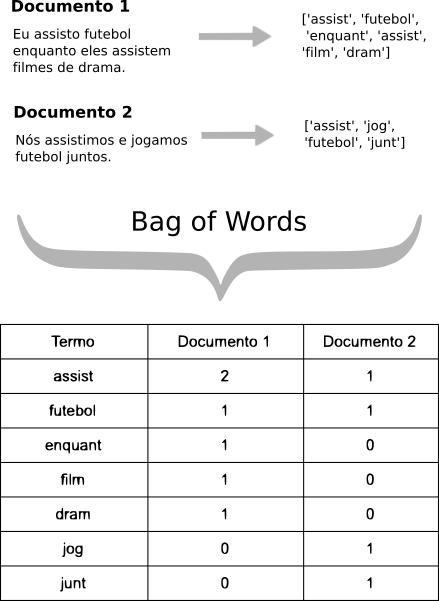
\includegraphics[width=0.7\textwidth]{figures/bag_of_words_example.png}
	\caption{Exemplo de representação \textit{bag of words}}
	\label{fig:bow_ex}
\end{figure}

\section{Word Embeddings}

Word embedding é a representação de palavras de um vocabulário em um espaço n-dimensional de números reais. Isso permite que palavras que são usadas de maneira similar tenham representações similares, de maneira a capturar o significado de cada palavra de acordo com a sua posição no espaço n-dimensional. Cada palavra é mapeada a um vetor e os valores desse vetor são obtidos a partir de um treinamentos que, em geral, envolvem redes neurais como o skip-gram utilizado na implementação word2vec, \cite{DBLP:journals/corr/MikolovSCCD13}.

\section{Redes Neurais Artificiais}

Redes Neurais são uma classe de funções em que a sua formulação matemática foi vagamente inspirada em estruturas biológicas do cérebro. Na analogia biológica dessa formulação, essas funções podem ser representadas no formato de um grafo em que as estruturas básicas são chamadas neurônios.

\begin{figure}[!ht]
	\centering
	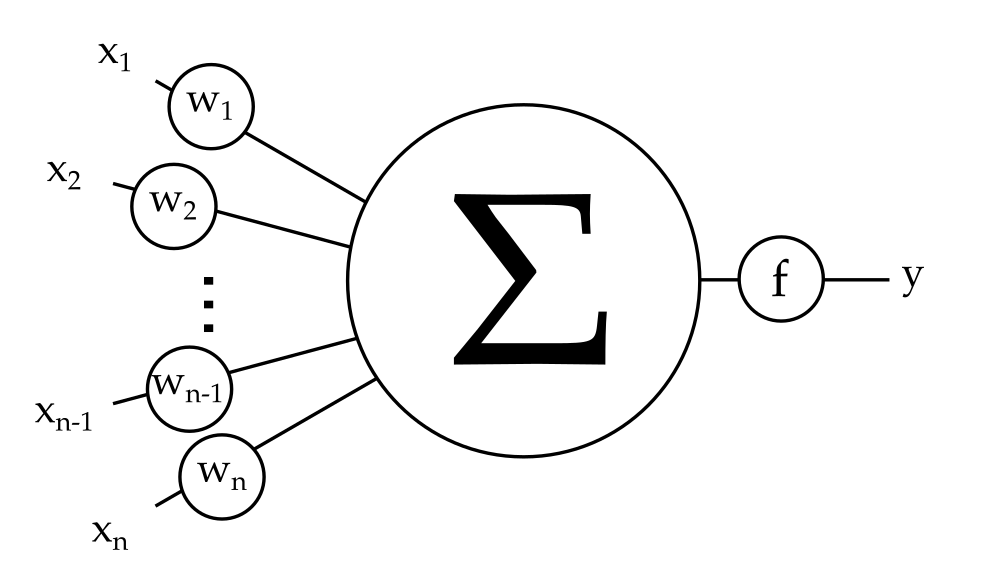
\includegraphics[width=0.6\textwidth]{figures/neuron.png}
	\caption{Neurônio artificial}
	\label{fig:neuron}
\end{figure}

Conforme a figura \ref{fig:neuron}, um neurônio artificial é uma função $y:\mathbb R^n \rightarrow \mathbb R$ com entrada $\vec x = <x_1,x_2,x_3,\dots,x_n>$ e saída $y = f(\sum\limits_{i=1}^n x_iw_i)$, em que $f$ é a chamada função de ativação, correspondendo tradicionalmente a função sigmoid, mas atualmente a função mais utilizada é a relu ($f(x) = max(0, x)$).

Os parâmetros que definem a arquitetura de uma rede neural tradicional dentro do conjunto da classe de funções são chamados hiperparâmetros. Esses parâmetros definem a quantidade de neurônios e as conexões entre eles que são tradicionalmente organizadas segundo camadas totalmente conectadas.

Uma característica que torna as redes neurais interessantes é o fato de elas atenderem ao Teorema da aproximação universal segundo \cite{HORNIK1991251}. Contudo, o que as tornam realmente especiais no contexto de aprendizado de máquinas é a maneira com que são encontrados os parâmetros para a aproximação de funções. Diferentemente da aproximação de funções diferenciáveis pelo teorema de Taylor por exemplo, existem heurísticas que permitem encontrar os parâmetros de uma rede neural para a aproximação da função a partir de amostras pontuais, i.e., dados, sem que seja necessário o conhecimento da função original como formulado no teorema de Taylor.

Dessa maneira, além dos hiperparâmetros, há as duas seguintes categorias de parâmetros em uma rede neural: parâmetros treináveis que são escolhidos a partir de procedimentos de treinamento envolvendo dados para a aproximação de funções; parâmetros de entrada que correspondem aos da função que se deseja aproximar. Uma vez encontrados parâmetros treináveis para uma aproximação satisfatória, estes são fixados e utilizam-se os parâmetros de entrada para realizar previsões nas situações de interesse.

Uma vez que a definição de parâmetros treináveis já foi realizada, pode-se retomar a análise das heurísticas que permitem determiná-los. Esse processo consiste em um algoritmo iterativo que minimiza uma função de custo baseada na comparação entre a saída da rede neural atual com dados de treinamento e os respectivos valores reais. Esse processo é chamado método do gradiente e, conforme o próprio nome diz, exige o cálculo do gradiente da função de custo em relação aos parâmetros treináveis e é viabilizado pelo algoritmo backpropagation por \cite{Rumelhart1986}. Atualmente, são utilizadas diversas técnicas para a otimização do método do gradiente \cite{DBLP:journals/corr/Ruder16}, envolvendo desde variações na forma como as variáveis são atualizadas no processo iterativo quanto como inicializar os parâmetros treináveis ou execuções em mini-batches.

\subsection{Redes Neurais Convolucionais}
Redes neurais convolucionais consistem em uma variação da arquitetura de redes neurais tradicionais em que parâmetros treináveis podem ser reutilizados em diferentes operações durante o cálculo de feedforward de uma rede neural. Isso permite o reconhecimento de um mesmo padrão em distintos subconjuntos dos dados de entrada, tornando esse tipo de arquitetura ideal para reconhecimento de objetos em imagens conforme originalmente descrito por \cite{LeCun1999}. Contudo, uma variação unidimensional da rede neural convolucional também pode ser útil no reconhecimento de padrões em textos com o auxílio de word embeddings.

\subsection{Redes Neurais Recorrentes}

Conforme ilustrado por \cite{ColahLSTM}, redes neurais recursivas são uma extensão das redes neurais tradicionais que visam permitir a representação de um estado de memória no processo de feedforward da rede. Isso é especialmente útil quando os dados de entrada dependem de uma sequência para possuírem coerência, como ocorre no caso de um texto. A extração máxima de informação de um texto só ocorre quando se leva em consideração a sequência das palavra, o que não é tratado no método bag of words por exemplo.

A representação de estado de memória em uma rede neural é viabilizada por meio de uma célula, i.e., um conjunto de neurônios com operações que são aplicadas uma vez para cada elemento da sequência de um dado de entrada. Dessa maneira, além de haver um compartilhamento de parâmetros treináveis como nas redes neurais convolucionais, também há um estado armazenado nos neurônios da célula que são realimentados a essa mesma célula ao executar as operações envolvendo o elemento seguinte da sequência, o que dá origem ao nome recorrente.

\chapter{Seleção do conjunto de dados e dos modelos}
\label{chapter:implementacaoResultados}
\noindent

\section{Seleção do Conjunto de Dados}

Neste trabalho, foram empregados dois modelos de representação de textos distintos. Cada modelo foi utilizado para gerar um descritor por questão com base no enunciado e alternativas. Esses descritores juntos aos rótulos de disciplina serviram de fonte de dados para modelos classificadores os quais foram comparados por meio de métricas como a acurácia.

Para estabelecer um padrão de comparação entre os distintos modelos, definiu-se um conjunto de parâmetros da API de dados descrita na seção \ref{dataset_api}. Dentre esses parâmetros, pode-se destacar o uso de um dicionário de agrupamento de assuntos conforme listado no apêndice \ref{JSON_dict} e um número mínimo de 10000 amostras por categoria de enunciado. A partir desses parâmetros, as 133 classes iniciais listadas no apêndice \ref{questoes_lista} foram reduzidas a apenas 9 classes conforme ilustra a figura \ref{fig:pie_labels_graph}.

\begin{figure}[!ht]
	\centering
	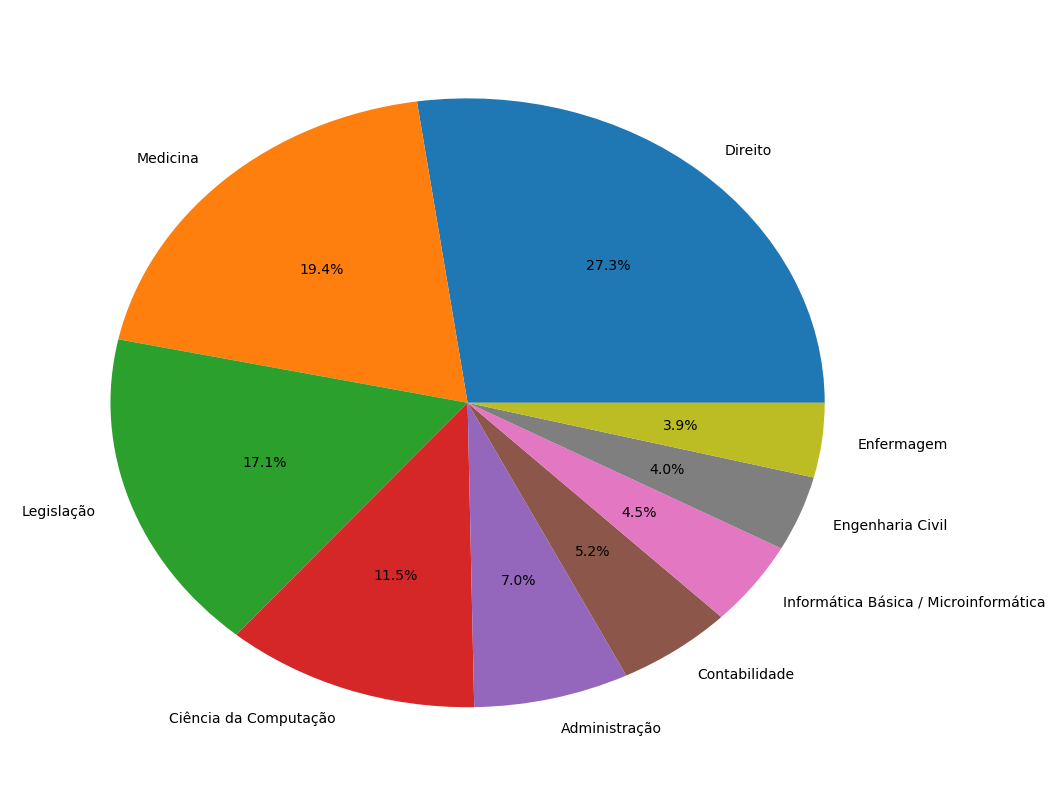
\includegraphics[width=1.0\textwidth]{figures/pie_graph.png}
	\caption{Distribuição das categorias selecionadas}
	\label{fig:pie_labels_graph}
\end{figure}

\section{Seleção dos Modelos}

Uma grande influência na escolha dos modelos em que foi dado um maior foco de otimização foi o guia de classificação de texto produzido por \cite{Text_classification_guide} e ilustrado pelo fluxograma da figura \ref{fig:TextClassificationFlowchart}. Esse guia se trata do resultado de anos de pesquisa em que foram executados cerca de 450 mil experimentos para avaliar a performance de diversos modelos com diferentes hiperparâmetros e conjuntos de dados. Assim, ele tem como objetivo evitar esforços redundantes na seleção e no treinamento de modelos em novos conjuntos de dados.

\begin{figure}[!ht]
	\centering
	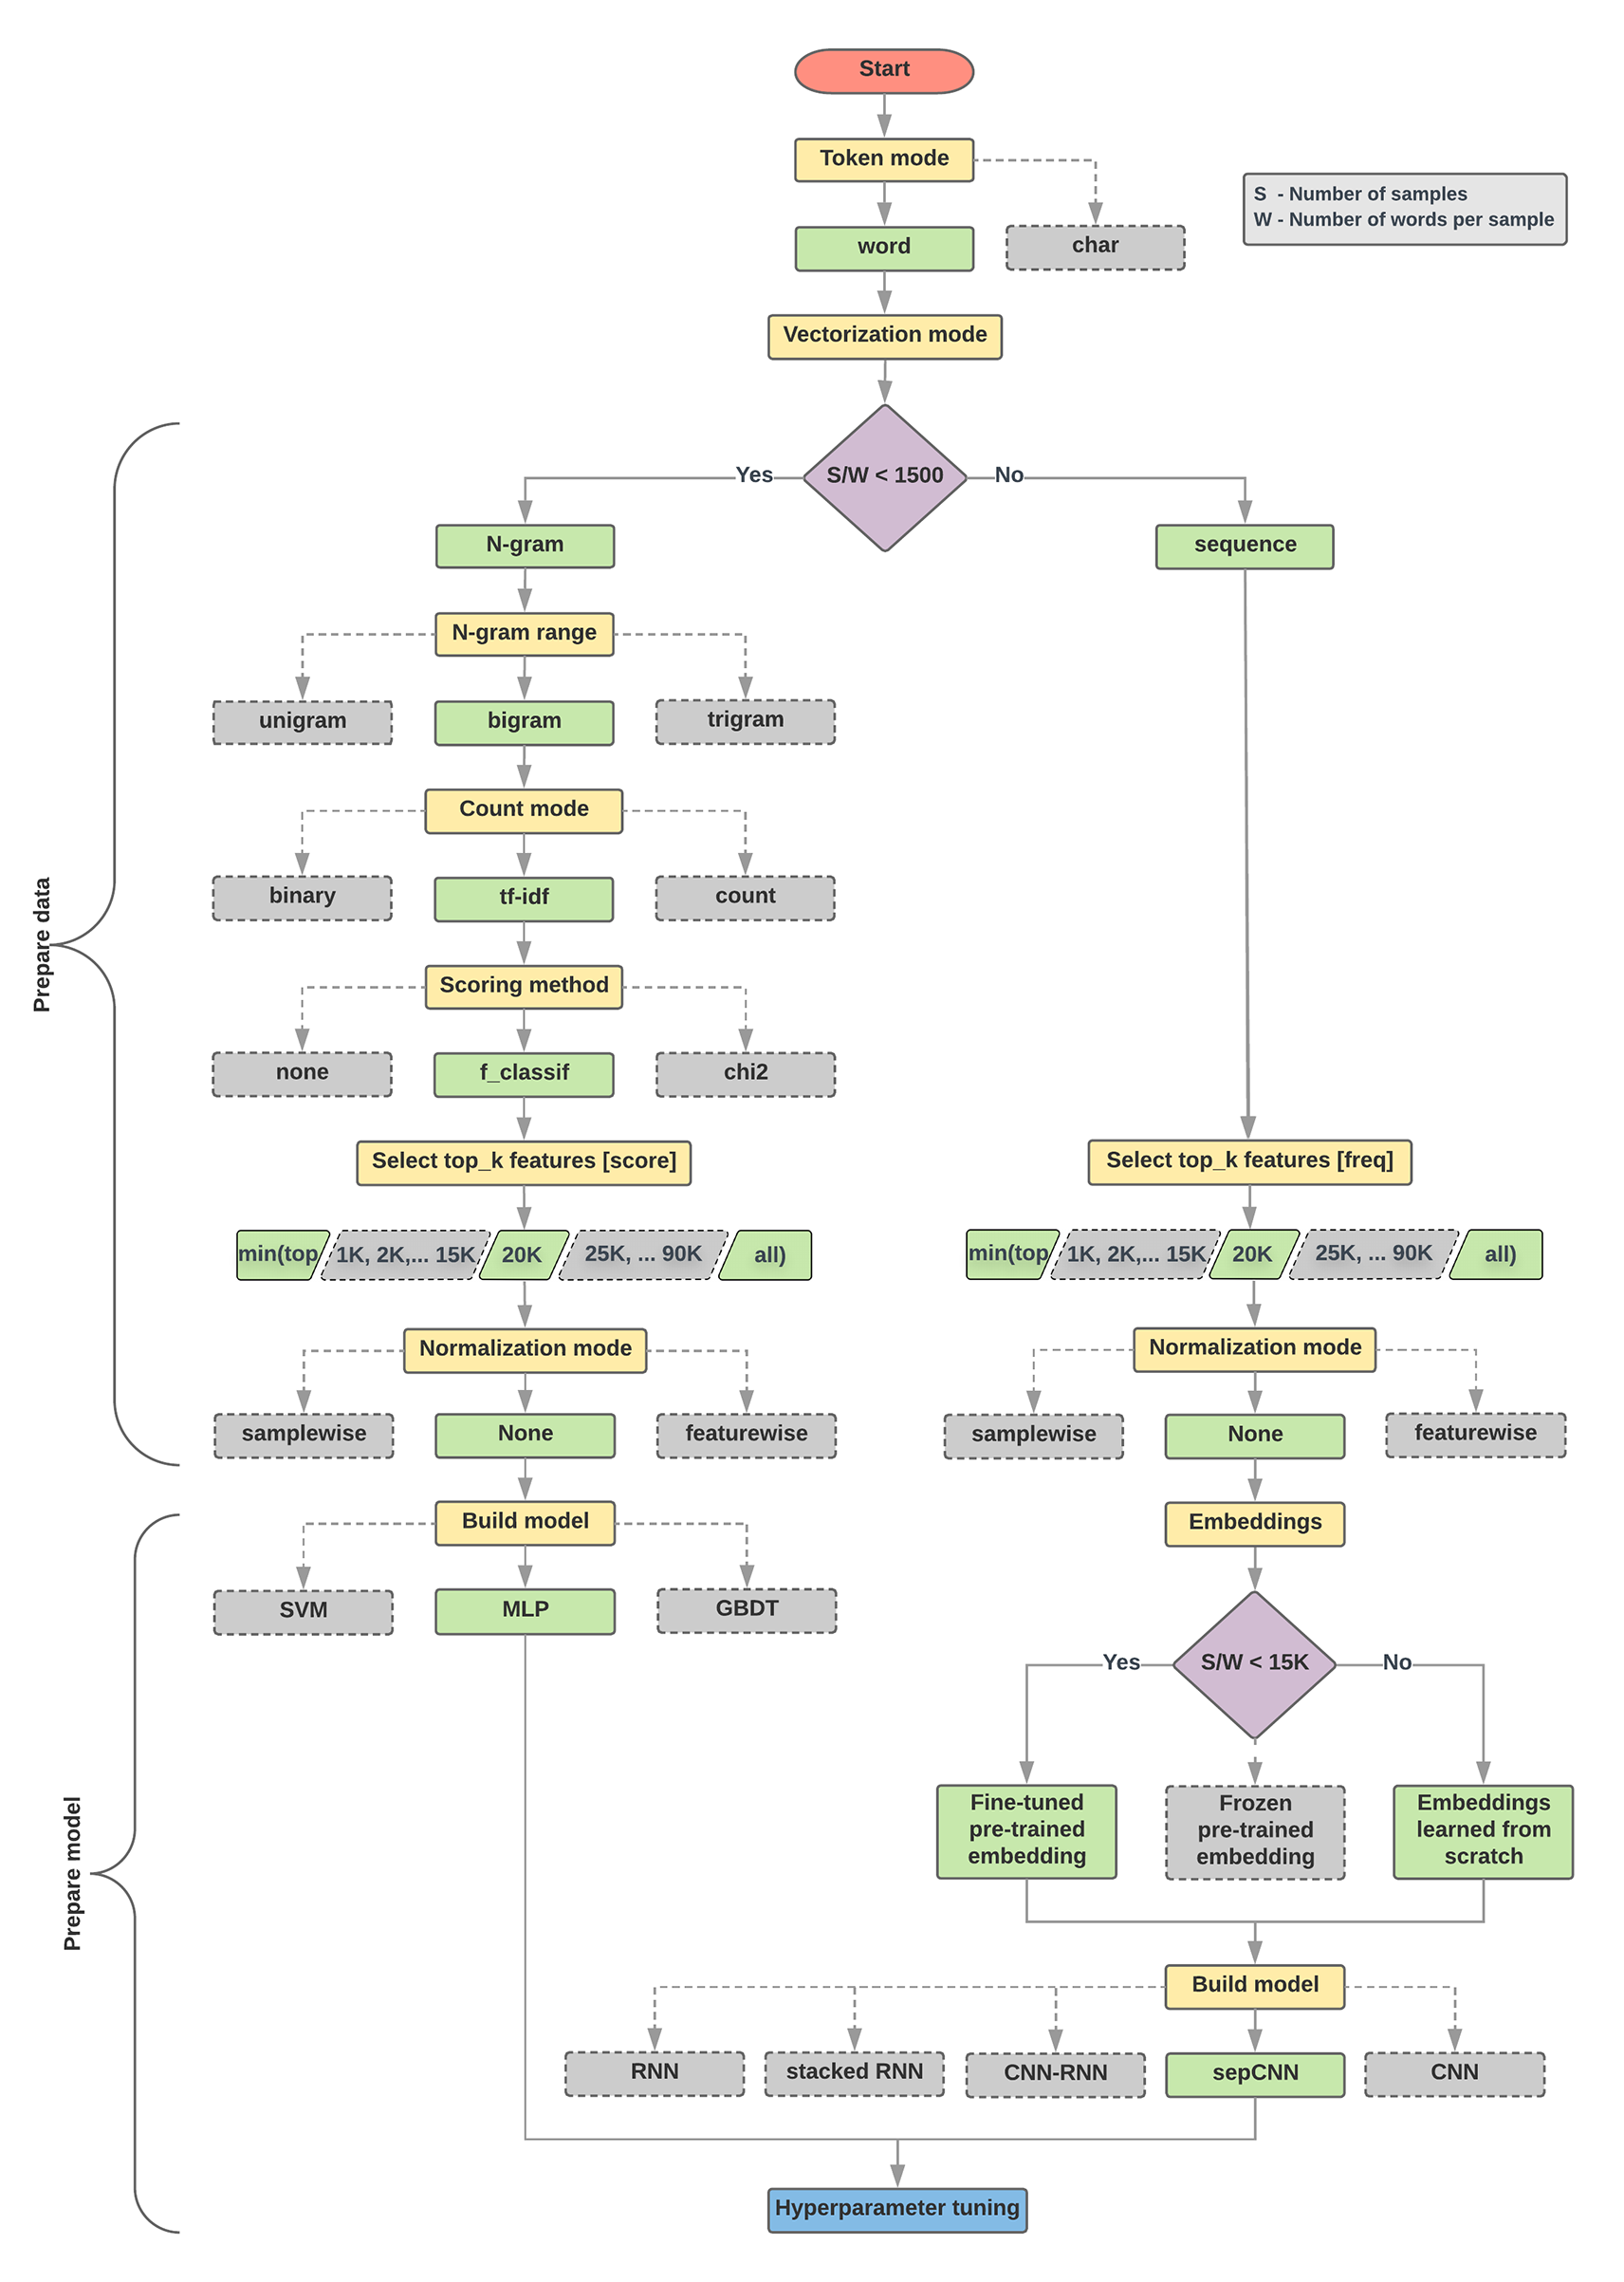
\includegraphics[width=1.0\textwidth]{figures/TextClassificationFlowchart.png}
	\caption{Fluxograma para classificação de texto (fonte: \cite{Text_classification_guide})}
	\label{fig:TextClassificationFlowchart}
\end{figure}

O fluxograma da figura \ref{fig:TextClassificationFlowchart} é baseado na correlação encontrada na razão entre o número de amostras do conjunto de dados (S) e a mediana do comprimento do texto de cada uma dessas questões (W) para a tomada de decisão em suas bifurcações na busca por uma acurácia ótima. No presente trabalho, a partir dos parâmetros da API de dados já definidos, tem-se um total de 299.314 amostras e uma mediana de 65 palavras por amostra, resultando em uma razão (S/W) de aproximadamente 4604.83. Assim, o modelo mais recomendado é o sequencial com o uso de \textit{word embedding} conforme ilustra a figura ref{fig:TextClassificationFlowchart}. Além disso, recomenda-se também o treinamento de uma camada de \textit{embedding} que parta de um modelo pré-treinado, pois um treinamento a partir de valores aleatórios exigiria uma maior razão S/W.

O presente trabalho não se restringe a modelos sequenciais. Implementou-se também modelos baseados em n-gramas, pois estes são modelos mais simples e tradicionais que atuam como bons pontos de referência na comparação dos resultados finais. Contudo, após uma avaliação inicial dos resultados, as recomendações do guia (por \cite{Text_classification_guide}) se confirmaram e os modelos sequenciais mostraram melhores resultados. Por essa razão, em iterações posteriores dos modelos, apenas os sequenciais foram explorados na busca por hiperparâmetros que correspondessem a melhores resultados.
%Cronograma
%• Deve estar presente apenas nos documentos parciais
%• Não aparece na versão final da monografia
%• Deve mostrar o andamento do projeto
%• Com possíveis atrasos
%• Deve ser específico para o trabalho
%• Nada de generalismos



% crawler
% interface
% simple machine learning
% - bag of words
% - simple avg
% deep learning
% - recurrent
% - convolutional
% integração com a plataforma

\chapter{Cronograma}


\begin{figure}[!ht]
	\centering
	\begin{ganttchart}{1}{12}
  \gantttitle{2018}{12} \\
  \gantttitlelist{1,...,12}{1} \\
  \ganttgroup{Pesquisa e configuração}{1}{4} \\
  \ganttbar{Pesquisa}{1}{4} \\
  \ganttbar{Configuração}{1}{2} \\
  
  \ganttmilestone{VE}{5}  \ganttnewline
  
  \ganttgroup{Implementação dos modelos}{5}{8} \\
  \ganttbar{Bag of Words}{5}{5} \\
  \ganttbar{Word Embedings}{5}{5} \\
  \ganttbar{Recurrent Neural Networks}{6}{8} \\
  \ganttbar{Convolutional Neural Networks}{6}{8} \\
  
  \ganttmilestone{VC}{8}  \ganttnewline
  
  \ganttgroup{Conclusão}{9}{10} \\
  \ganttbar{Avaliação dos resultados}{9}{9}\\
  \ganttbar{Integração com o loona}{9}{12}\\

  \ganttmilestone{VF}{10} \ganttnewline
  
  \ganttlink{elem0}{elem3}
  \ganttlink{elem3}{elem4}
  
  \ganttlink{elem4}{elem9}
  \ganttlink{elem9}{elem10}
  
  \ganttlink{elem10}{elem13}
\end{ganttchart} 
	\caption{Diagrama de Gantt}
	\label{fig:gantt}
\end{figure}




% -----
% PARTE DE REFERÊCIAS BIBLIOGRÁFICAS DE PFC
%
%  As referências do documento de PFC devem estar no arquivo refs.bib
%  Devem seguir o formato bibtex - ver Manual-Referencias.pdf para mais detalhes.
% -----
\bibliographystyle{pfc}
\bibliography{refs}

% -----
% PARTE DE APÊNDICE DE PFC
%
%  Se o documento de PFC não tiver apêndices REMOVER AS LINHAS ABAIXO
%  Adicionar os arquivos .tex de apêndice ao documento com comando \include{•}
% -----
\inappendix
%%
%
% ARQUIVO: apendice.tex
%
% VERSÃO: 1.0
% DATA: Maio de 2016
% AUTOR: Coordenação de Trabalhos Especiais SE/8
% 
%  Arquivo tex de exemplo de apêndice do documento de Projeto de Fim de Curso.
%  Este exemplo traz dois apêndices (dois comandos \chapter{•}). Poderiam ser colocados em arquivos .tex
%  separados. Neste caso, o arquivo main.tex deveria ter um \include{•} para cada arquivo .tex
%
% ---
% DETALHES
%  a. todo apêndice deve começar com \chapter{•}
%  b. usar comando \noindent logo após \chapter{•}
%  c. segue os mesmos DETALHES do arquivo .tex de exemplo de capítulo do documento de Projeto de Fim de Curso
% ---
%%
\chapter{Apêndice Exemplo}
\noindent
Curabitur tortor. Pellentesque nibh. Aenean quam. In scelerisque sem at dolor. Maecenas mattis. Sed convallis tristique sem. Proin ut ligula vel nunc egestas porttitor. Morbi lectus risus, iaculis vel, suscipit quis, luctus non, massa. Fusce ac turpis quis ligula lacinia aliquet. Mauris ipsum. Nulla metus metus, ullamcorper vel, tincidunt sed, euismod in, nibh. Quisque volutpat condimentum velit.

Class aptent taciti sociosqu ad litora torquent per conubia nostra, per inceptos himenaeos. Nam nec ante. Sed lacinia, urna non tincidunt mattis, tortor neque adipiscing diam, a cursus ipsum ante quis turpis. Nulla facilisi. Ut fringilla. Suspendisse potenti. Nunc feugiat mi a tellus consequat imperdiet. Vestibulum sapien. Proin quam. Etiam ultrices. Suspendisse in justo eu magna luctus suscipit. Sed lectus. Integer euismod lacus luctus magna.

Lorem ipsum dolor sit amet, consectetur adipiscing elit. Integer nec odio. Praesent libero. Sed cursus ante dapibus diam. Sed nisi. Nulla quis sem at nibh elementum imperdiet. Duis sagittis ipsum. Praesent mauris. Fusce nec tellus sed augue semper porta. Mauris massa. Vestibulum lacinia arcu eget nulla. Class aptent taciti sociosqu ad litora torquent per conubia nostra, per inceptos himenaeos. Curabitur sodales ligula in libero. Sed dignissim lacinia nunc.

\chapter{Apêndice Exemplo 02}
\noindent
Curabitur tortor. Pellentesque nibh. Aenean quam. In scelerisque sem at dolor. Maecenas mattis. Sed convallis tristique sem. Proin ut ligula vel nunc egestas porttitor. Morbi lectus risus, iaculis vel, suscipit quis, luctus non, massa. Fusce ac turpis quis ligula lacinia aliquet. Mauris ipsum. Nulla metus metus, ullamcorper vel, tincidunt sed, euismod in, nibh. Quisque volutpat condimentum velit.

Class aptent taciti sociosqu ad litora torquent per conubia nostra, per inceptos himenaeos. Nam nec ante. Sed lacinia, urna non tincidunt mattis, tortor neque adipiscing diam, a cursus ipsum ante quis turpis. Nulla facilisi. Ut fringilla. Suspendisse potenti. Nunc feugiat mi a tellus consequat imperdiet. Vestibulum sapien. Proin quam. Etiam ultrices. Suspendisse in justo eu magna luctus suscipit. Sed lectus. Integer euismod lacus luctus magna.

Lorem ipsum dolor sit amet, consectetur adipiscing elit. Integer nec odio. Praesent libero. Sed cursus ante dapibus diam. Sed nisi. Nulla quis sem at nibh elementum imperdiet. Duis sagittis ipsum. Praesent mauris. Fusce nec tellus sed augue semper porta. Mauris massa. Vestibulum lacinia arcu eget nulla. Class aptent taciti sociosqu ad litora torquent per conubia nostra, per inceptos himenaeos. Curabitur sodales ligula in libero. Sed dignissim lacinia nunc.

\outappendix

% -----
% PARTE DE ANEXO DE PFC
%
%  Se o documento de PFC não tiver anexos REMOVER AS LINHAS ABAIXO
%  Adicionar os arquivos .tex de anexo ao documento com comando \include{•}
% -----
\inannex
%%
%
% ARQUIVO: anexo.tex
%
% VERSÃO: 1.0
% DATA: Maio de 2016
% AUTOR: Coordenação de Trabalhos Especiais SE/8
% 
%  Arquivo tex de exemplo de anexo do documento de Projeto de Fim de Curso.
%  Este exemplo traz dois anexos (dois comandos \chapter{•}). Poderiam ser colocados em arquivos .tex
%  separados. Neste caso, o arquivo main.tex deveria ter um \include{•} para cada arquivo .tex
%
% ---
% DETALHES
%  a. todo anexo deve começar com \chapter{•}
%  b. usar comando \noindent logo após \chapter{•}
%  c. segue os mesmos DETALHES do arquivo .tex de exemplo de capítulo do documento de Projeto de Fim de Curso
% ---
%%
% \chapter{Anexo Exemplo}
% \noindent
% Id magna feugiat. Erat pellentesque sapien in rhoncus dolor augue vel eget. Erat nibh animi ultricies sit rhoncus. Eleifend aliquam luctus sem turpis habitasse. Lectus arcu ut mi nulla luctus facilisis cursus suspendisse class sociis metus vitae leo consequat lorem ullamcorper arcu. Nunc justo aliquam. Quidem volutpat urna. Nonummy nulla blandit donec vitae ultrices. Netus aliquam vivamus. Vehicula libero leo. Vestibulum consectetuer magna. Sapien aliquam arcu netus etiam lectus. Venenatis tristique morbi non nulla tortor commodo gravida ac neque lacinia urna. Elit mauris adipisci. Vitae sed curabitur. Tellus nunc lectus. Nonummy et integer.
% 
% Lorem dictumst enim. Dui vestibulum quisque. Dolor posuere risus. Nullam vitae est magnis est tortor metus dolor integer. Massa elit nec euismod et lacus quam ac malesuada est suspendisse ut est pellentesque vivamus lorem amet non vulputate maecenas et id ultrices lacus odio morbi vitae ac aenean in feugiat elit sodales congue proin dui leo bibendum scelerisque faucibus in suscipit. Nulla parturient in. Eget habitasse fringilla. Eget donec excepturi wisi lorem lacinia. Elementum lorem sem. Pede metus sit. Aenean facilisi pellentesque. Purus dictum ante. Neque amet sed.
% 
% Sed leo molestie. Elit fusce placerat lectus quis aliquam nulla turpis platea. Integer mus bibendum sed wisi pretium ullamcorper nunc arcu. Ipsum maecenas sed. Et pariatur in. Ut wisi non. Bibendum nec et quisque quam diam sed dolor lorem. Pellentesque fames donec senectus nulla purus dui nibh praesent. Pariatur nulla augue sapien elit imperdiet aliquam ullamcorper orci. Integer nec mauris. Sit magnis vel ut leo a sapien proin at. Etiam sem aliquam bibendum mauris purus ac sagittis ultrices. Mollis eleifend est. Nec vitae posuere at arcu purus. In elementum vehicula.
% 
% \chapter{Anexo Exemplo 02}
% \noindent
% Id magna feugiat. Erat pellentesque sapien in rhoncus dolor augue vel eget. Erat nibh animi ultricies sit rhoncus. Eleifend aliquam luctus sem turpis habitasse. Lectus arcu ut mi nulla luctus facilisis cursus suspendisse class sociis metus vitae leo consequat lorem ullamcorper arcu. Nunc justo aliquam. Quidem volutpat urna. Nonummy nulla blandit donec vitae ultrices. Netus aliquam vivamus. Vehicula libero leo. Vestibulum consectetuer magna. Sapien aliquam arcu netus etiam lectus. Venenatis tristique morbi non nulla tortor commodo gravida ac neque lacinia urna. Elit mauris adipisci. Vitae sed curabitur. Tellus nunc lectus. Nonummy et integer.
% 
% Lorem dictumst enim. Dui vestibulum quisque. Dolor posuere risus. Nullam vitae est magnis est tortor metus dolor integer. Massa elit nec euismod et lacus quam ac malesuada est suspendisse ut est pellentesque vivamus lorem amet non vulputate maecenas et id ultrices lacus odio morbi vitae ac aenean in feugiat elit sodales congue proin dui leo bibendum scelerisque faucibus in suscipit. Nulla parturient in. Eget habitasse fringilla. Eget donec excepturi wisi lorem lacinia. Elementum lorem sem. Pede metus sit. Aenean facilisi pellentesque. Purus dictum ante. Neque amet sed.
% 
% Sed leo molestie. Elit fusce placerat lectus quis aliquam nulla turpis platea. Integer mus bibendum sed wisi pretium ullamcorper nunc arcu. Ipsum maecenas sed. Et pariatur in. Ut wisi non. Bibendum nec et quisque quam diam sed dolor lorem. Pellentesque fames donec senectus nulla purus dui nibh praesent. Pariatur nulla augue sapien elit imperdiet aliquam ullamcorper orci. Integer nec mauris. Sit magnis vel ut leo a sapien proin at. Etiam sem aliquam bibendum mauris purus ac sagittis ultrices. Mollis eleifend est. Nec vitae posuere at arcu purus. In elementum vehicula.
% 
\outannex

% -----
% FIM DO DOCUMENTO DE PFC
% -----
\label{theend}
\end{document}
